\documentclass[11pt]{report}
\usepackage[margin=2.5cm]{geometry}
\usepackage[french]{babel}
\usepackage[T1]{fontenc}
\usepackage[explicit]{titlesec}
\usepackage{times}
\usepackage{fancyhdr}
\usepackage{graphicx}
\usepackage{ucs}
\usepackage[utf8x]{inputenc}
\usepackage{awesomebox}
\usepackage{fontawesome5}
\setmainfont{Liberation Serif}

\titleformat{\chapter}[display]{\Huge}{\thechapter. #1}{20pt}{\small}

\titlespacing{\chapter}{0pt}{.1cm}{.1cm}

\lhead[\rightmark]{\rightmark}
\chead[]{}
\rhead[\thepage]{\thepage}

\lfoot[]{}
\cfoot[\thepage]{\thepage}
\rfoot[]{}

\renewcommand{\headrulewidth}{0.5pt}

\pagestyle{fancy}

\begin{document}
\begin{titlepage}
   \begin{center}
       \vspace*{5cm}

       \Huge\textbf{Manuel utilisateur}

       \vspace{0.5cm}
       \Large


       Moteur 3D - 7Physics


       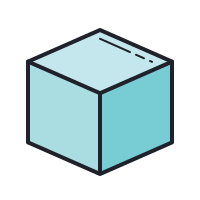
\includegraphics[width=2cm]{./logo.png}

       \vspace{1cm}

       \large
       \textbf{Équipe 3 : Noa AMMIRATI, Fanny DELNONDEDIEU, Quentin GENDARME, Pierre LOTTE, Théo PIROUELLE, Éléa TURC}

       \vfill

       
\includegraphics[width=15cm]{./enseeiht.jpeg}

       \vspace{2cm}

       ENSEEIHT\\
       Département Sciences du Numérique\\
       1APP SN 2020-2021


   \end{center}
\end{titlepage}


\tableofcontents


\chapter{Manipuler des objets 3D}

\section{Ajouter un objet 3D}
Pour pouvoir ajouter un objet 3D sur la scène 3D, il faut sur la partie droite de l'interface, sélectionner en haut la forme souhaitée.\newline \newline
\notebox{Pour afficher un \textbf{cube} sur la scène 3D, il faut sélectionner le bouton : 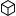
\includegraphics[width=0.4cm]{./btn_cube.png}\newline
Pour afficher d'autres formes, il suffit de sélectionner les boutons adjacents. }

\section{Supprimer un objet 3D}


\chapter{Déplacer la caméra}

\section{Zoomer}
\awesomebox{\faKeyboard}{5pt}{cyan}{ Il est possible de zoomer à l'aide du clavier grâce aux commandes ...}
\newline
\awesomebox{\faMousePointer}{5pt}{teal}{Il est possible de zoomer avec la souris ...}

\section{Dezoomer}
\awesomebox{\faKeyboard}{5pt}{lightgray}{Test de couleurs ...}
\newline
\awesomebox{\faMousePointer}{5pt}{lime}{...}

\section{Avancer sur la scène}
\awesomebox{\faKeyboard}{5pt}{blue}{...}
\newline
\awesomebox{\faMousePointer}{5pt}{pink}{...}

\section{Reculer sur la scène}
\awesomebox{\faKeyboard}{5pt}{violet}{...}
\newline
\awesomebox{\faMousePointer}{5pt}{orange}{...}

\section{Tourner}
\awesomebox{\faKeyboard}{5pt}{brown}{...}
\newline
\awesomebox{\faMousePointer}{5pt}{darkgray}{...}

\end{document}
